\documentclass{beamer}
\usepackage[italian]{babel}
\usepackage[utf8]{inputenc}

\usetheme{Copenhagen} 
\usecolortheme{crane}

\title[avifauna.fem2ambiente]{Sviluppo e-commerce\\avifauna.fem2ambiente.com}
\author[Mattia Curatitoli]{\textbf{Mattia Curatitoli} \and \\[1cm] 
	Relatore: \textbf{Prof. Daniela Micucci} \and \\
	Correlatore: \textbf{Dr. Emanuele Ferri}}
\date{Ottobre 2015}

% --personal definitions--
\def \fem {FEM2-Ambiente}
\def \sv {Sviluppo Portale Avifauna}
\def \wp {WordPress}
\def \js {JavaScript}

\begin{document}

\begin{frame}
 \maketitle
\end{frame}

\begin{frame}
 \begin{center}
  {\huge FEM2 - Ambiente}\\[1cm]
  \begin{columns}
   \column{0.60\textwidth}
    \begin{center}
	 Uno spin-off del Dipartimento di Biotecnologie e Bioscienze dell'Università degli studi di Milano-Bicocca \\[0.5cm]
     La mission dell'azienda è creare prodotti e servizi per il largo pubblico finalizzati alla conoscenza e tutela della biodiversità.    
    \end{center}
   \column{0.39\textwidth}
   \begin{figure}
    
\includegraphics[scale=0.7]{images/fem}
   \end{figure}
  \end{columns}
 \end{center}
\end{frame}

\begin{frame}
 \frametitle{\fem}
 \begin{center}
  La crescita di {\fem} sul mercato ha portato alla creazione del sito dedicato \url{www.fem2ambiente.com} \\ 
  dove è presente un e-commerce per la vendita di prodotti per l'analisi di acqua ed eco-prodotti per la casa \\[1cm]
  {\fem} offre anche servizi di analisi su avifauna \\
  La prima soluzione per la gesitione degli ordini è stata attraverso fogli elettronici Excel \\
  La crescita della clientela ha richiesto lo sviluppo di una piattaforma dedicata
 \end{center}
\end{frame}

\begin{frame}
 \begin{center}
  {\huge Sviluppo Portale Avifauna}
 \end{center}
\end{frame}

\begin{frame}
 \frametitle{\sv}
 \begin{center}
  Struttura sito \\www.avifauna.fem2ambiente.com \\
  \begin{figure}
    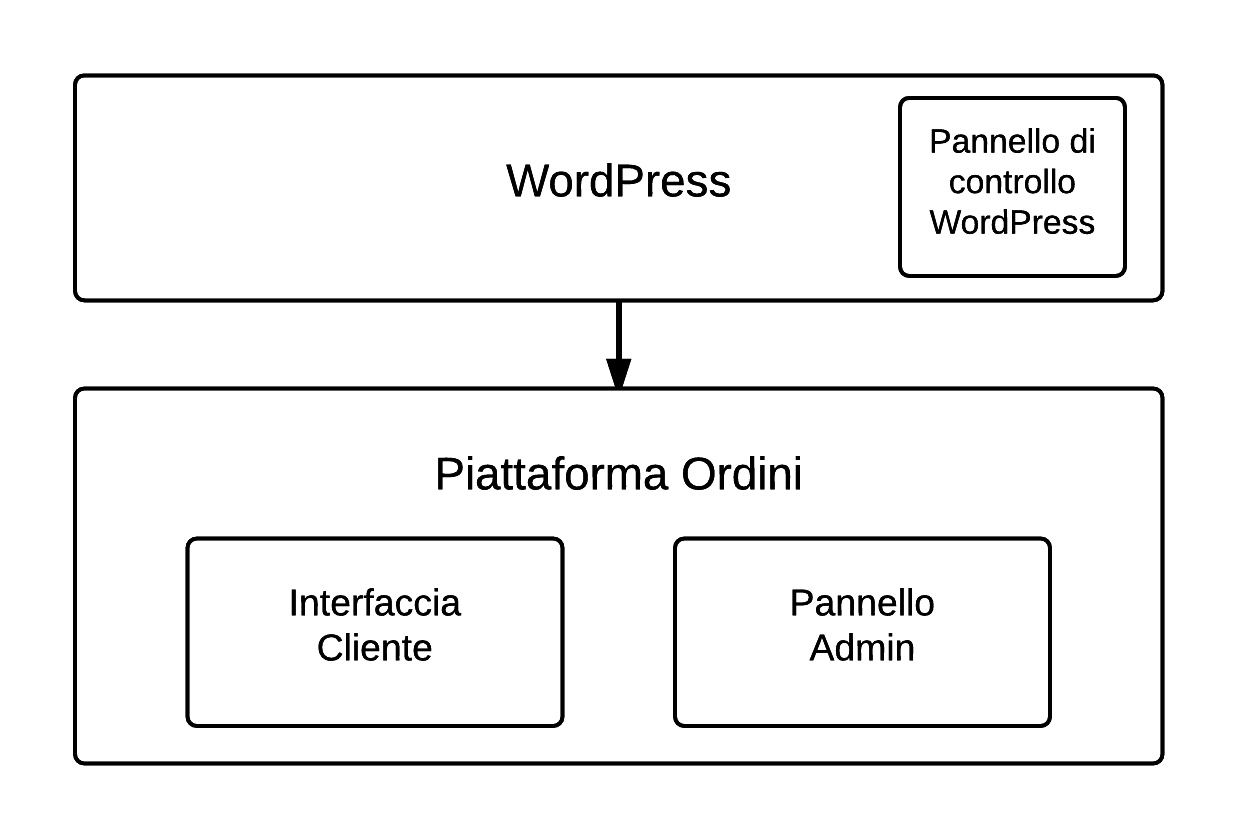
\includegraphics[scale=0.9]{images/struttura-sito}
  \end{figure}
 \end{center}
\end{frame}

\begin{frame}
 \frametitle{\sv}
 \begin{center}
  \begin{columns}
   \column{0.60\textwidth}
   \begin{center}
     {\wp} è un CMS \\
     Content Management System \\
     facile da usare \\
     personalizzabile con temi e plugin
   \end{center}
   \column{0.35\textwidth}
   \begin{figure}
     
\includegraphics[scale=0.12]{images/wordpress}
   \end{figure}
  \end{columns}
 \end{center}
\end{frame}

\begin{frame}
 \frametitle{\sv}
 \begin{center}
  Struttura piattaforma degli ordini
  \begin{columns}
   \column{0.09\textwidth}
   \column{0.35\textwidth}
    Lato front-end:
     \begin{itemize}
      \item HTML
      \item CSS
      \item {\js}
     \end{itemize}
    Lato server:
     \begin{itemize}
      \item Django
     \end{itemize}
   \column{0.55\textwidth}
   \begin{figure}
     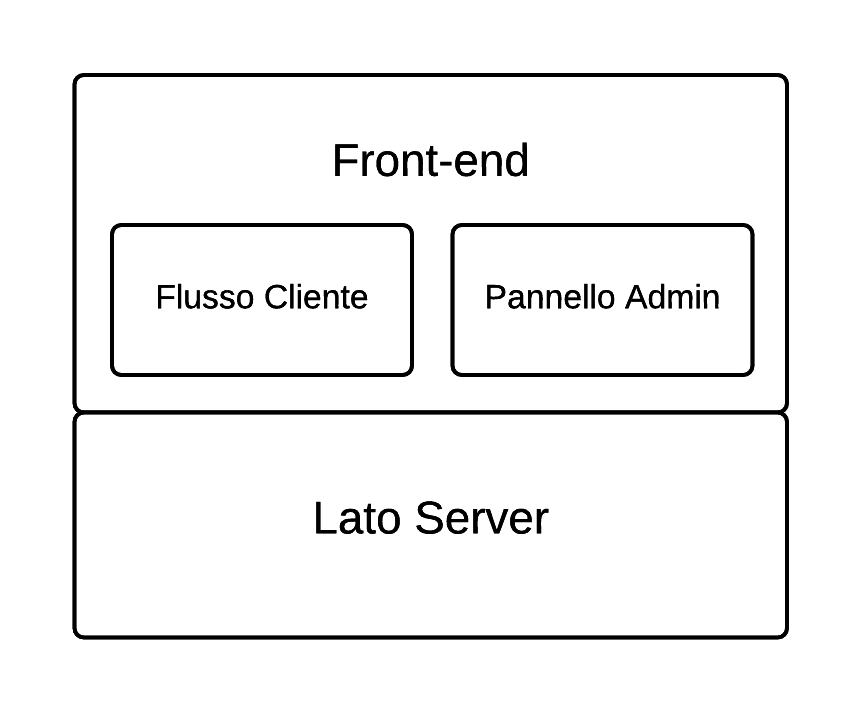
\includegraphics[scale=0.75]{images/struttura-piattaforma}
   \end{figure}
  \end{columns}
 \end{center}
\end{frame}

\begin{frame}
 \frametitle{\sv}
 \begin{center}
  \begin{columns}
   \column{0.55\textwidth}
   \begin{center}
    \textbf{\emph{Lato Server}} : \\[0.5cm]
    Django, un web framework scritto in Python
   \end{center}
   \column{0.40\textwidth}
   \begin{figure}
     
\includegraphics[scale=0.08]{images/django}
   \end{figure}
  \end{columns}
 \end{center}
\end{frame}

\begin{frame}
 \frametitle{\sv}
 \begin{center}
  \begin{columns}
   \column{0.45\textwidth}
   \begin{center}
	 La struttura è composta da \emph{modelli} connessi tra loro come classi java \\[0.5cm]
	 completato da un sistema per la gestione multilingua
   \end{center}
   \column{0.55\textwidth}
   \begin{figure}
     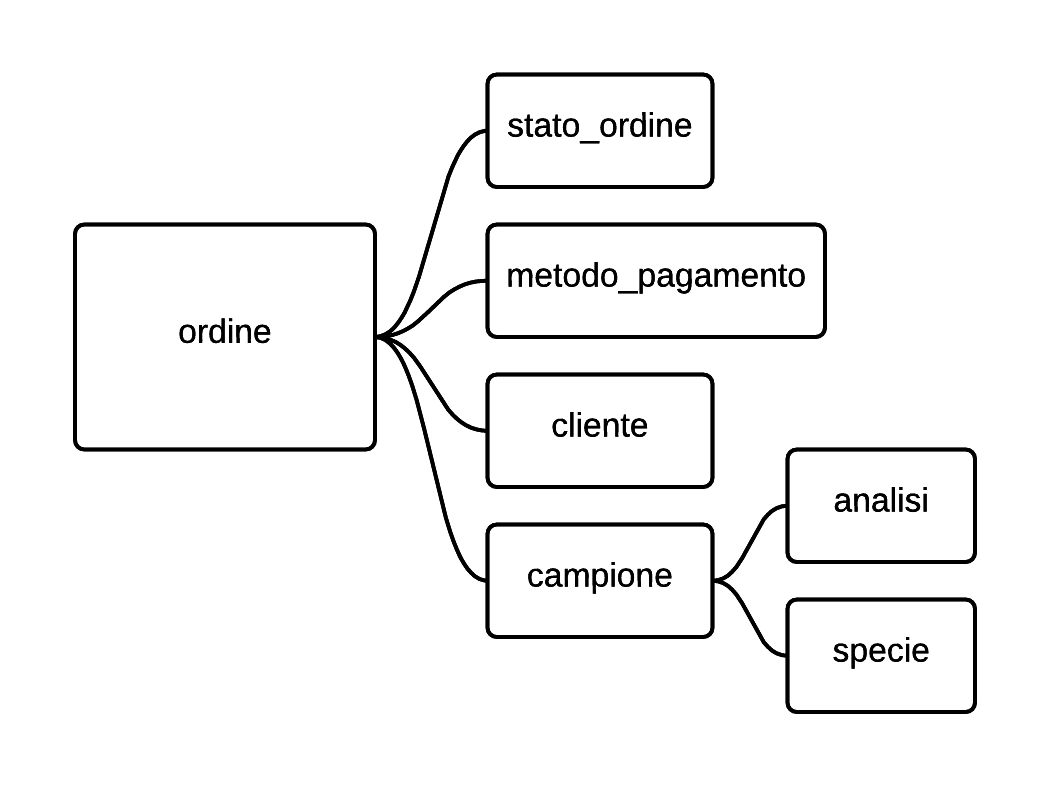
\includegraphics[scale=0.65]{images/modelli}
   \end{figure}
  \end{columns}
 \end{center}
\end{frame}

\begin{frame}
 \frametitle{\sv}
 \begin{center}
  \begin{columns}
   \column{0.55\textwidth}
   \begin{center}
    \textbf{\emph{Lato Front-end}} : \\[0.5cm]
    \begin{itemize}
     \item HTML, linguaggio di markup per la formattazione e impaginazione di pagine web
     \item CSS, linguaggio per la formattazione di documenti HTML
     \item JavaScript, linguaggio di scripting lato client per personalizzazione di pagine web
     \item Bootstrap, framework composto da modelli in HTML, CSS e {\js}
    \end{itemize}
   \end{center}
   \column{0.40\textwidth}
   \begin{figure}
     
\includegraphics[scale=0.25]{images/html5-js-css3}
   \end{figure}
   \begin{figure}
     
\includegraphics[scale=0.3]{images/bootstrap}
   \end{figure}
  \end{columns}
 \end{center}
\end{frame}

\begin{frame}
 \frametitle{Flusso Cliente}
 \begin{center}
  {\huge Flusso Cliente}
  \begin{columns}
   \column{0.49\textwidth}
    \begin{figure}
      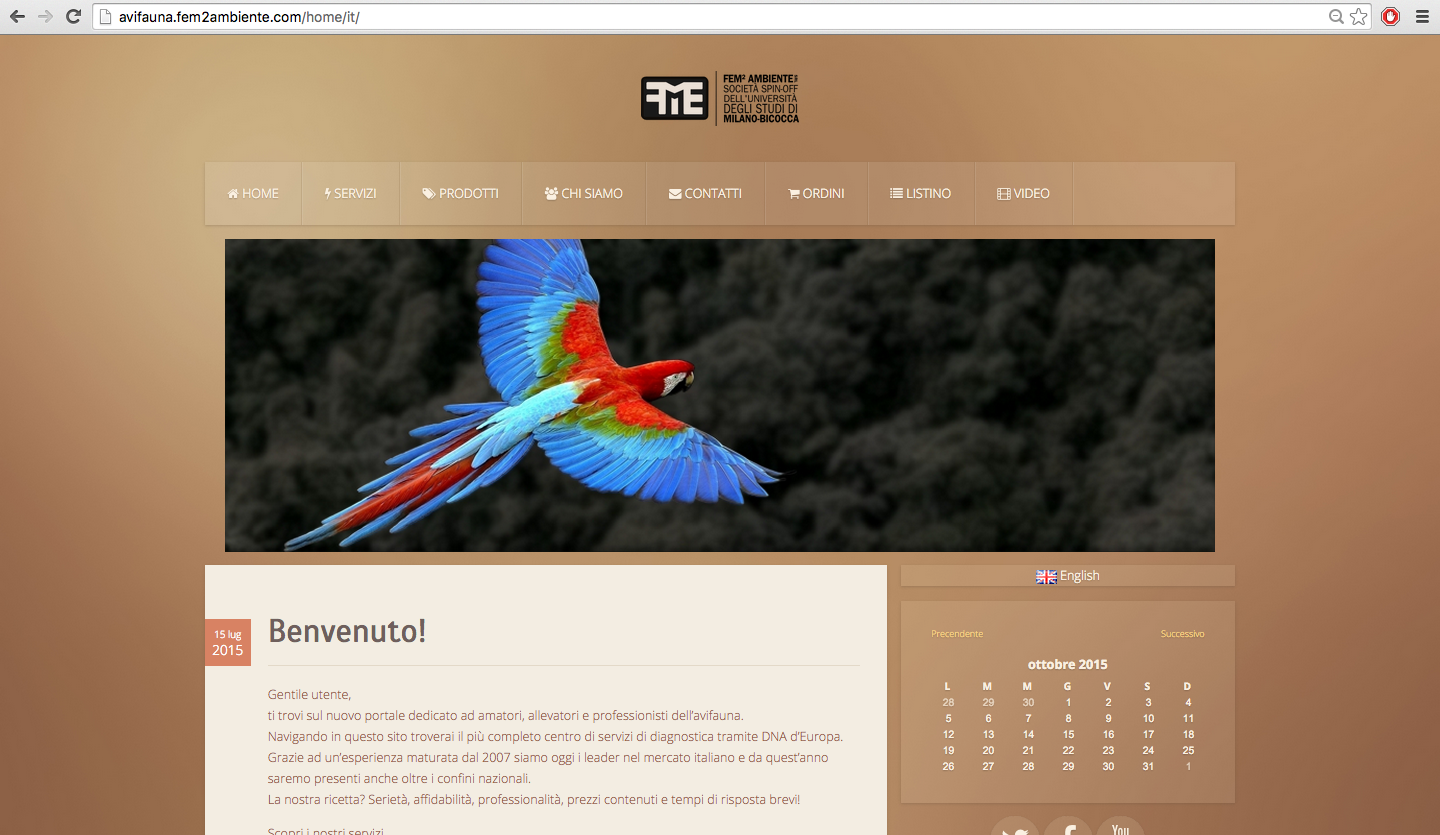
\includegraphics[scale=0.1]{images/cl-homepage-wp}
    \end{figure} 
    homepage di WordPress
   \column{0.49\textwidth}
    \begin{figure}
      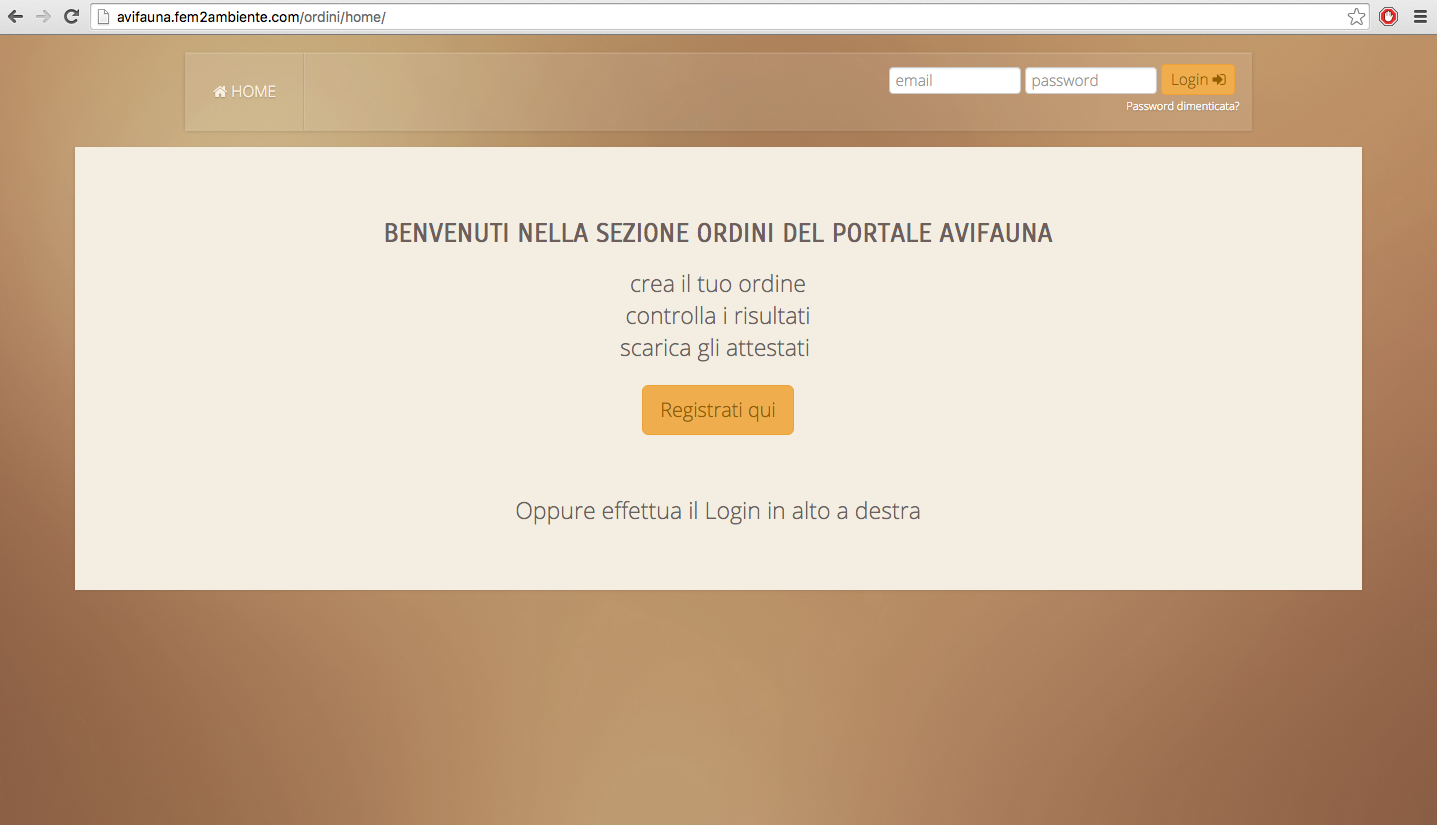
\includegraphics[scale=0.1]{images/cl-homepage-p2}
    \end{figure} 
    homepage della piattaforma
  \end{columns}
 \end{center}
\end{frame}

\begin{frame}
 \frametitle{Flusso Cliente}
 \begin{center}
  \begin{figure}
    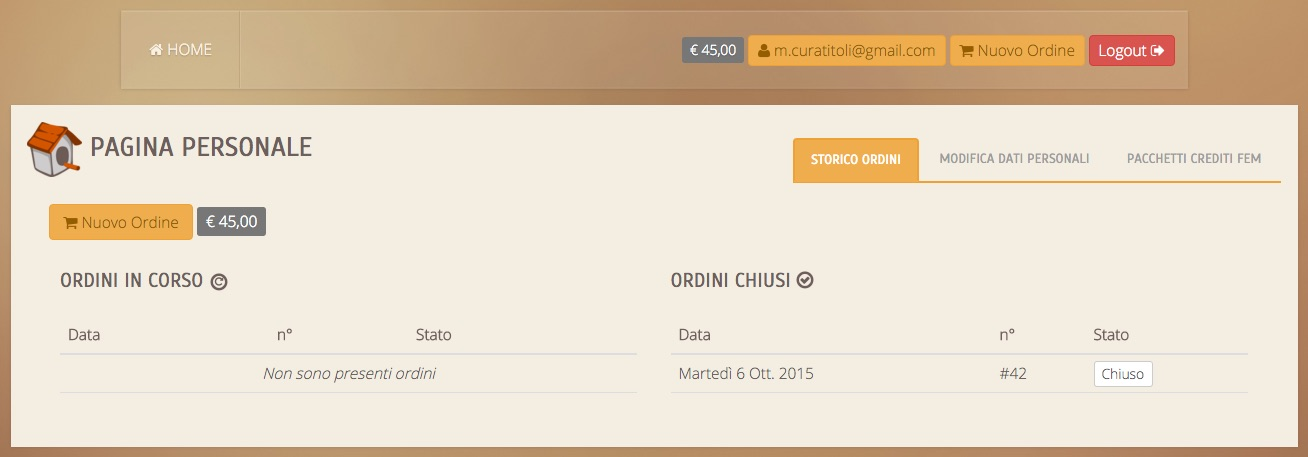
\includegraphics[scale=0.2]{images/cl-pagina-personale}
  \end{figure} 
  pagina personale
  \begin{figure}
    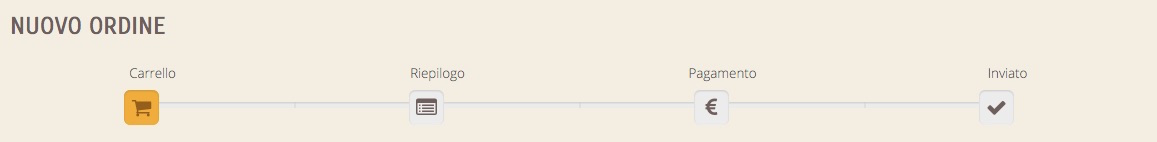
\includegraphics[scale=0.2]{images/cl-nuovo-ordine-bar}
  \end{figure} 
  nuovo ordine
 \end{center}
\end{frame}

\begin{frame}
 \frametitle{Flusso Cliente}
 \begin{center}
  \begin{figure}
    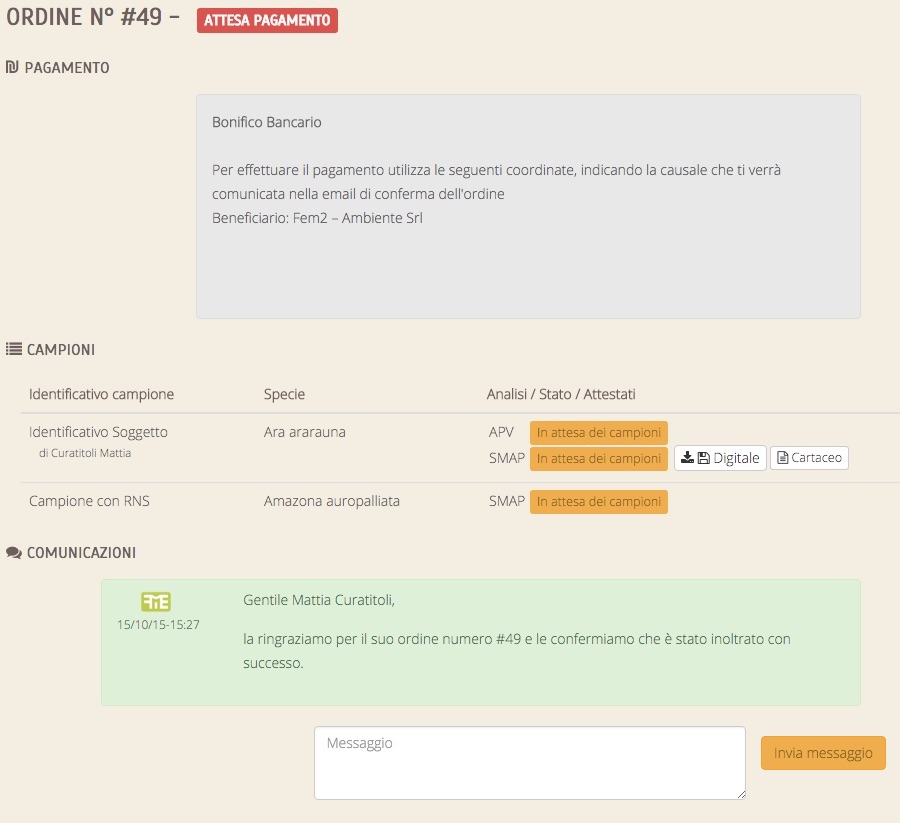
\includegraphics[scale=0.2]{images/cl-ordine}
  \end{figure} 
  pagina ordine
 \end{center}
\end{frame}

\begin{frame}
 \frametitle{Flusso Amministratore}
 \begin{center}
  {\huge Flusso Amministratore}
  \begin{columns}
   \column{0.39\textwidth}
    \begin{figure}
      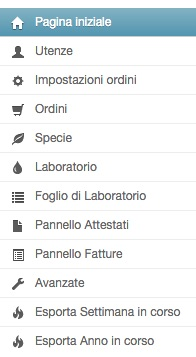
\includegraphics[scale=0.4]{images/admin-navbar}
    \end{figure} 
   \column{0.60\textwidth}
   \begin{center}
 	Pannello admin di Django personalizzato per gestire al meglio il flusso dell'ordine e del cliente
   \end{center}
  \end{columns}
 \end{center}
\end{frame}

\begin{frame}
 \frametitle{Flusso Amministratore}
 \begin{center}
  \begin{figure}
    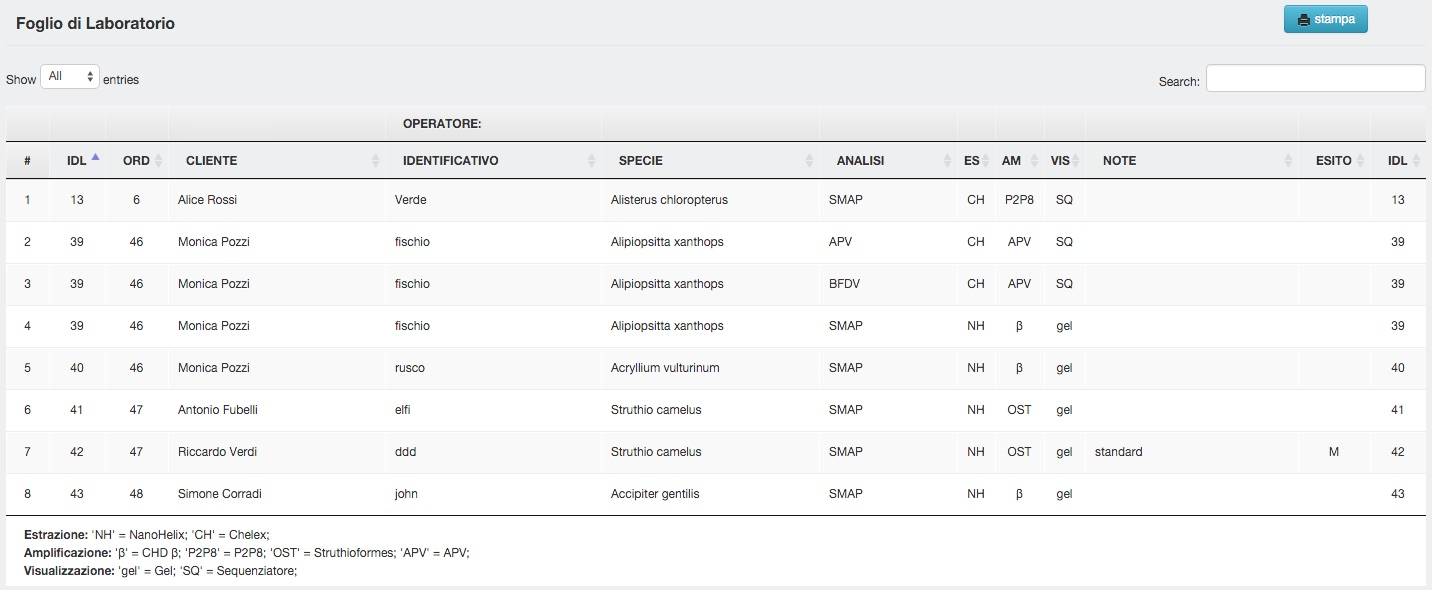
\includegraphics[scale=0.2]{images/admin-fogliolab-tab}
  \end{figure} 
  tabella per il foglio di laboratorio
 \end{center}
\end{frame}

\begin{frame}
 \begin{center}
  \begin{figure}
    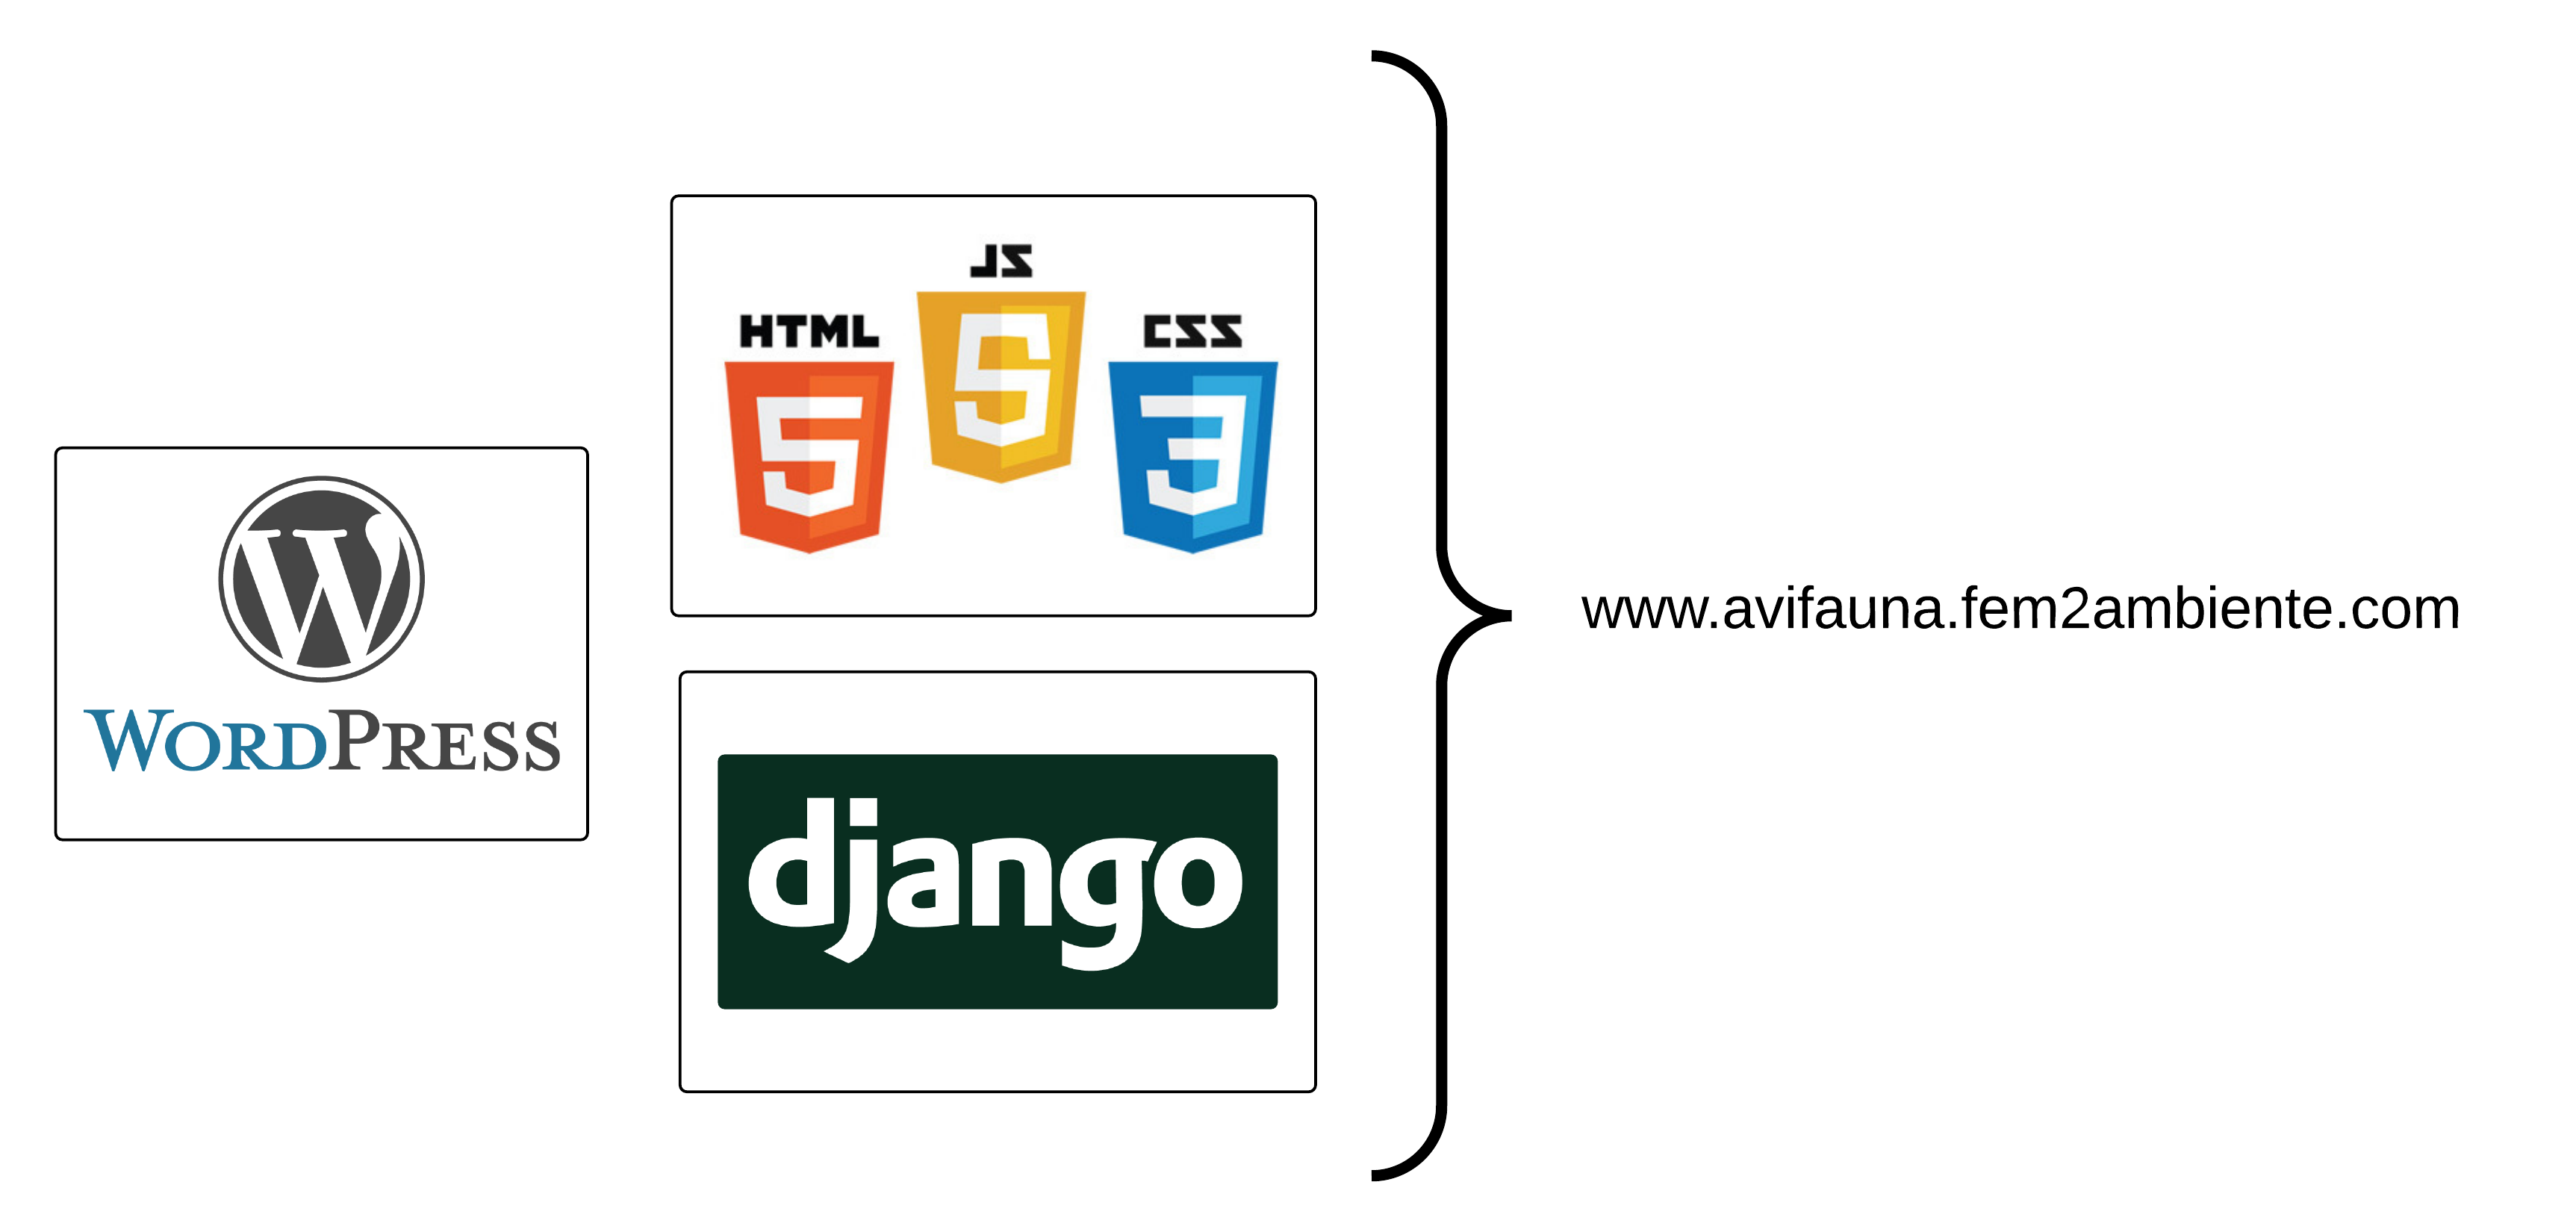
\includegraphics[scale=0.35]{images/conclusione}
  \end{figure} 
 \end{center}
\end{frame}

\end{document}
